\section{DSP}


\begin{frame}{Inlets para DSP}
\begin{figure}[h!]
\centering
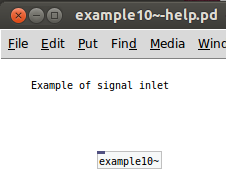
\includegraphics[width=0.5\textwidth]{example10}
\caption{Primeiro Inlet DSP}
\end{figure}
\end{frame}


\begin{frame}{Inlets para DSP}
Alguns pontos importantes:
\begin{itemize}
\item Existem macros para facilitar a definição do primeiro inlet para classes
do tipo \texttt{CLASS\_DEFAULT}.
\item Inlets adicionais são instanciados no método \texttt{\_new()}.
\end{itemize}
\end{frame}


\begin{frame}{Código para o primeiro inlet DSP (1/2)}
{Estrutura e métodos \texttt{\_perform()} e \texttt{\_dsp()}}
\lstinputlisting[name=Exemplo 10,linerange={6-9,22-29,30-34}]{../examples/src/example10.c}
\end{frame}


\begin{frame}{Código para o primeiro inlet DSP (2/2)}
{Método \texttt{\_setup()}}
\lstinputlisting[name=Exemplo 10,linerange={36-46},firstnumber=last]{../examples/src/example10.c}
\end{frame}


\begin{frame}{Inlets DSP adicionais (1/2)}
{Método \texttt{\_new()}}
\lstinputlisting[linerange={12-19},firstnumber=last]{../examples/src/example11.c}
\end{frame}


\begin{frame}{Inlets DSP adicionais (2/2)}
{Métodos \texttt{\_perform()} e \texttt{\_dsp()}}
\lstinputlisting[linerange={26-38}]{../examples/src/example11.c}
\end{frame}


\begin{frame}{Inlets DSP adicionais}
\begin{figure}[h!]
\centering
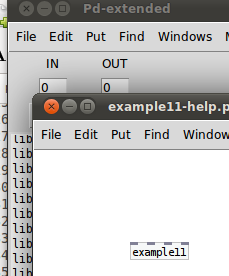
\includegraphics[width=0.5\textwidth]{example11}
\end{figure}
\end{frame}


\begin{frame}{Outlets DSP}
{Método \texttt{\_new()}}
\lstinputlisting[linerange={12-20}]{../examples/src/example12.c}
\end{frame}


\begin{frame}{Outlets DSP}
\begin{figure}[h!]
\centering
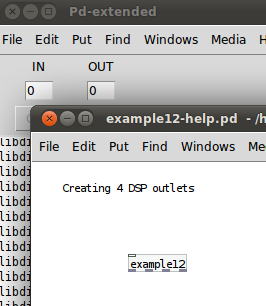
\includegraphics[width=0.5\textwidth]{example12}
\end{figure}
\end{frame}


\begin{frame}{Inlets e outlets criados dinamicamente}
\textbf{Cenário:} o objeto possui um número de inlets (e outlets) igual a um parâmetro
passado no momento de sua criação. 
\end{frame}


\begin{frame}{Inlets e outlets criados dinamicamente (1/3)}
{Estrutura e método \texttt{\_dsp()}}
\lstinputlisting[linerange={6-10,44-48}]{../examples/src/example17.c}
\end{frame}


\begin{frame}{Inlets e outlets criados dinamicamente (2/3)}
{Método \texttt{\_new()}}
\lstinputlisting[linerange={12-25},firstnumber=last]{../examples/src/example17.c}
\end{frame}


\begin{frame}{Inlets e outlets criados dinamicamente (3/3)}
{Método \texttt{\_perform()}}
\lstinputlisting[linerange={33-43},firstnumber=last]{../examples/src/example17.c}
\end{frame}
